\PassOptionsToPackage{unicode=true}{hyperref} % options for packages loaded elsewhere
\PassOptionsToPackage{hyphens}{url}
%
\documentclass[]{article}
\usepackage{lmodern}
\usepackage{amssymb,amsmath}
\usepackage{ifxetex,ifluatex}
\usepackage{fixltx2e} % provides \textsubscript
\ifnum 0\ifxetex 1\fi\ifluatex 1\fi=0 % if pdftex
  \usepackage[T1]{fontenc}
  \usepackage[utf8]{inputenc}
  \usepackage{textcomp} % provides euro and other symbols
\else % if luatex or xelatex
  \usepackage{unicode-math}
  \defaultfontfeatures{Ligatures=TeX,Scale=MatchLowercase}
\fi
% use upquote if available, for straight quotes in verbatim environments
\IfFileExists{upquote.sty}{\usepackage{upquote}}{}
% use microtype if available
\IfFileExists{microtype.sty}{%
\usepackage[]{microtype}
\UseMicrotypeSet[protrusion]{basicmath} % disable protrusion for tt fonts
}{}
\IfFileExists{parskip.sty}{%
\usepackage{parskip}
}{% else
\setlength{\parindent}{0pt}
\setlength{\parskip}{6pt plus 2pt minus 1pt}
}
\usepackage{hyperref}
\hypersetup{
            pdftitle={Statistical Learning Final Project: Predicting Country HDI},
            pdfauthor={Daniel Alonso},
            pdfborder={0 0 0},
            breaklinks=true}
\urlstyle{same}  % don't use monospace font for urls
\usepackage[margin=1in]{geometry}
\usepackage{graphicx,grffile}
\makeatletter
\def\maxwidth{\ifdim\Gin@nat@width>\linewidth\linewidth\else\Gin@nat@width\fi}
\def\maxheight{\ifdim\Gin@nat@height>\textheight\textheight\else\Gin@nat@height\fi}
\makeatother
% Scale images if necessary, so that they will not overflow the page
% margins by default, and it is still possible to overwrite the defaults
% using explicit options in \includegraphics[width, height, ...]{}
\setkeys{Gin}{width=\maxwidth,height=\maxheight,keepaspectratio}
\setlength{\emergencystretch}{3em}  % prevent overfull lines
\providecommand{\tightlist}{%
  \setlength{\itemsep}{0pt}\setlength{\parskip}{0pt}}
\setcounter{secnumdepth}{0}
% Redefines (sub)paragraphs to behave more like sections
\ifx\paragraph\undefined\else
\let\oldparagraph\paragraph
\renewcommand{\paragraph}[1]{\oldparagraph{#1}\mbox{}}
\fi
\ifx\subparagraph\undefined\else
\let\oldsubparagraph\subparagraph
\renewcommand{\subparagraph}[1]{\oldsubparagraph{#1}\mbox{}}
\fi

% set default figure placement to htbp
\makeatletter
\def\fps@figure{htbp}
\makeatother

\usepackage{xcolor}

\title{Statistical Learning Final Project: Predicting Country HDI}
\author{Daniel Alonso}
\date{December 19th, 2020}

\begin{document}
\maketitle

{
\setcounter{tocdepth}{4}
\tableofcontents
}
\newpage

\hypertarget{dataset-of-choice}{%
\section{Dataset of choice}\label{dataset-of-choice}}

For this project I decided to pick a custom-built dataset obtained from
the \href{https://databank.worldbank.org/home.aspx}{World bank
Databank}, specifically the
\href{https://databank.worldbank.org/source/world-development-indicators}{World
Development Indicators database}. This is the ``primary World Bank
collection of development indicators'' as stated on the database
description. It has lots of economic, education, energy use, and
population specific metrics.

I find demographic data fascinating, and I think this dataset will be
quite good for predicting country development measures along with
providing quite interesting and relevant information.

\hypertarget{variables}{%
\subsection{Variables}\label{variables}}

\large

NOTE: \normalsize

\begin{itemize}
\tightlist
\item
  \textbf{\textcolor{blue}{blue}} = used for training/predicting
\item
  \textbf{\textcolor{red}{red}} = target variable
\item
  \textbf{\textcolor{green}{green}} = ID variables
\item
  \textbf{\textcolor{violet}{purple}} = variables excluded as either
  they were \emph{components} of HDI or they were 100\% correlated to
  another variable (like GNI/GDP, which are both 100\% correlated and
  GNI is a component of HDI)
\end{itemize}

Variables in the original dataset as constructed using the World Bank
Databank tool (variables were renamed):

\begin{itemize}
\tightlist
\item
  \textcolor{green}{\textbf{year}}: year the data was obtained in
\item
  \textcolor{green}{\textbf{year\_code}}: code for the year as the world
  bank databank sets it
\item
  \textcolor{green}{\textbf{country\_name}}: name of the country
\item
  \textcolor{green}{\textbf{country\_code}}: alpha-3 ISO 3166 code for
  the country
\item
  \textcolor{blue}{\textbf{foreign\_inv\_inflows}}: Foreign direct
  investment, net inflows (BoP, current US\$)
\item
  \textcolor{blue}{\textbf{exports\_perc\_gdp}}: Exports of goods and
  services (as a \% of GDP)
\item
  \textcolor{blue}{\textbf{inflation\_perc}}: Inflation, consumer prices
  (annual \%)
\item
  \textcolor{blue}{\textbf{education\_years}}: Compulsory education,
  duration (years)
\item
  \textcolor{blue}{\textbf{education\_perc\_gdp}}: Government
  expenditure on education, total (as a \% of GDP)
\item
  \textcolor{blue}{\textbf{gds\_perc\_gdp}}: Gross domestic savings (as
  a \% of GDP)
\item
  \textcolor{blue}{\textbf{gross\_savings\_perc\_gdp}}: Gross savings
  (as a \% of GDP)
\item
  \textcolor{blue}{\textbf{int\_tourism\_arrivals}}: International
  tourism, number of arrivals
\item
  \textcolor{blue}{\textbf{int\_tourism\_receipts}}: International
  tourism, receipts (in current US\$)
\item
  \textcolor{blue}{\textbf{perc\_internet\_users}}: Individuals using
  the Internet (as a \% of population)
\item
  \textcolor{blue}{\textbf{access\_to\_electricity}}: Access to
  electricity (\% of population)
\item
  \textcolor{blue}{\textbf{agricultural\_land}}: Agricultural land (\%
  of land area)
\item
  \textcolor{blue}{\textbf{birth\_rate}}: Birth rate, crude (per 1,000
  people)
\item
  \textcolor{blue}{\textbf{gne}}: Gross national expenditure (\% of GDP)
\item
  \textcolor{blue}{\textbf{mobile\_subscriptions}}: Mobile cellular
  subscriptions (per 100 people)
\item
  \textcolor{blue}{\textbf{infant\_mort\_rate}}: Mortality rate, infant
  (per 1,000 live births)
\item
  \textcolor{blue}{\textbf{sex\_ratio}}: Sex ratio at birth (male births
  per female births)
\item
  \textcolor{blue}{\textbf{greenhouse\_gas\_em}}: Total greenhouse gas
  emissions (kt of CO2 equivalent)
\item
  \textcolor{blue}{\textbf{urban\_pop\_perc}}: Urban population (\% of
  total population)
\item
  \textcolor{red}{\textbf{hdi}}: human development index
\item
  \textcolor{red}{\textbf{hdi\_cat}}: Human development index as a
  category
\item
  \textcolor{violet}{\textbf{life\_exp}}: Life expectancy at birth,
  total (years)
\item
  \textcolor{violet}{\textbf{gdp}}: GDP (current US\$)
\item
  \textcolor{violet}{\textbf{gni}}: GNI (current US\$)
\item
  \textcolor{violet}{\textbf{fertility\_rate}}: Fertility rate, total
  (births per woman)
\end{itemize}

\newpage

\hypertarget{the-target-variable}{%
\subsubsection{The target variable}\label{the-target-variable}}

As all these variables could perhaps tell us how developed a country is,
we used a constructed categorized Human development index variable in
order to classify the countries using the above variables (unless stated
otherwise by their colour) as training variables.

The criteria for constructing the categorical variable \emph{hdi\_cat}
was the following:

\begin{itemize}
    \item Very high: HDI above 0.8
    \item High: HDI between 0.7 and 0.799
    \item Medium: HDI between 0.55 and 0.699
    \item Low: HDI under 0.55
  \end{itemize}

This categorization is emulated from Wikipedia's construction and uses
the same ranges as used in every Wikipedia article referencing HDI.

\hypertarget{data-preprocessing}{%
\section{Data preprocessing}\label{data-preprocessing}}

The data cleanup and preliminary feature engineering was done in Python
and the imputation was then done in R within the same Jupyter Notebook
(called \emph{preprocessing.ipynb}).

\hypertarget{methodology-and-steps}{%
\subsection{Methodology and steps}\label{methodology-and-steps}}

\begin{enumerate}
  \item Prior to importing there was a search within the .csv file with the following regex: \begin{verbatim} \s\[[\w\S]{1,}\] \end{verbatim} as a find and replace and removing every instance of it. This regex matches a metadata tag that the world bank uses in their dataset. Following this step, the data was imported.

  \item Metadata at the end of the dataset was removed, the dataset was filtered excluding these region codes (the codes were excluded as they were country aggregates, and we're only interested in the countries themselves).

  \item The year column was converted to integer and the '..' values (which represent NAs in the World bank databank) were replaced for numpy NaNs and then the values were sorted by year and country name.

  \item Data missing in later years (2020, 2019) was backfilled with data from previous years, as it still fits our modelling purposes. The data that goes the furthest back is from ~18 years prior, so 2002.

  \item Columns with more than 45 NA values were removed as this represents roughly 25% of the countries in question.

  \item The life expectancy, GDP, GNI and fertility rate columns were removed as these are either components of HDI or (in the case of fertility rate) are 100% correlated with other elements in our dataset (crude birth rate in this particular case).

  \item We scrape Wikipedia in order to obtain an updated metric on HDI estimates for each country. We also scrape it to obtain the alpha-3 3166 codes for each country. The data was obtained with the purpose of making it easier to join with the dataset obtained from the World Bank, as joining by country names is not reliable enough (misses ~20 countries which the alpha-3 codes do not).

  \item We add HDI to the main dataframe

  \item Numerical columns were converted into floats and column names were simplified for easier future manipulation.

  \item The categorical target variable is constructed as explained previously in this step.

  \item The data is then exported as a csv, along with a json file that shows how the columns were renamed

  \item The data is then imported in an R cell and a MICE imputation is performed using the 'cart' method with m = 5 in order to impute the very few missing values remaining.
\end{enumerate}

\newpage

\hypertarget{exploratory-data-analysis}{%
\section{Exploratory Data Analysis}\label{exploratory-data-analysis}}

\hypertarget{looking-at-variables-by-themselves}{%
\subsection{Looking at variables by
themselves}\label{looking-at-variables-by-themselves}}

The plots of choice for visually analyzing the variables prior to any
processing has been Boxplots and Histograms/density plots all looked at
individually and categorized by \emph{hdi\_cat} which is our categorical
target variable (HDI).

Given the space constraints of this report, if a plot for a specific
variable is not shown here but talked about or mentioned, it will be
shown in the \emph{eda.ipynb} and \emph{eda.html} notebook and notebook
export used to perform the visual analysis. Only variables which are
used in the modelling section will be visually analyzed and described.

\hypertarget{significantly-right-skewed-variables}{%
\subsubsection{Significantly right-skewed
variables}\label{significantly-right-skewed-variables}}

\begin{figure}
\centering
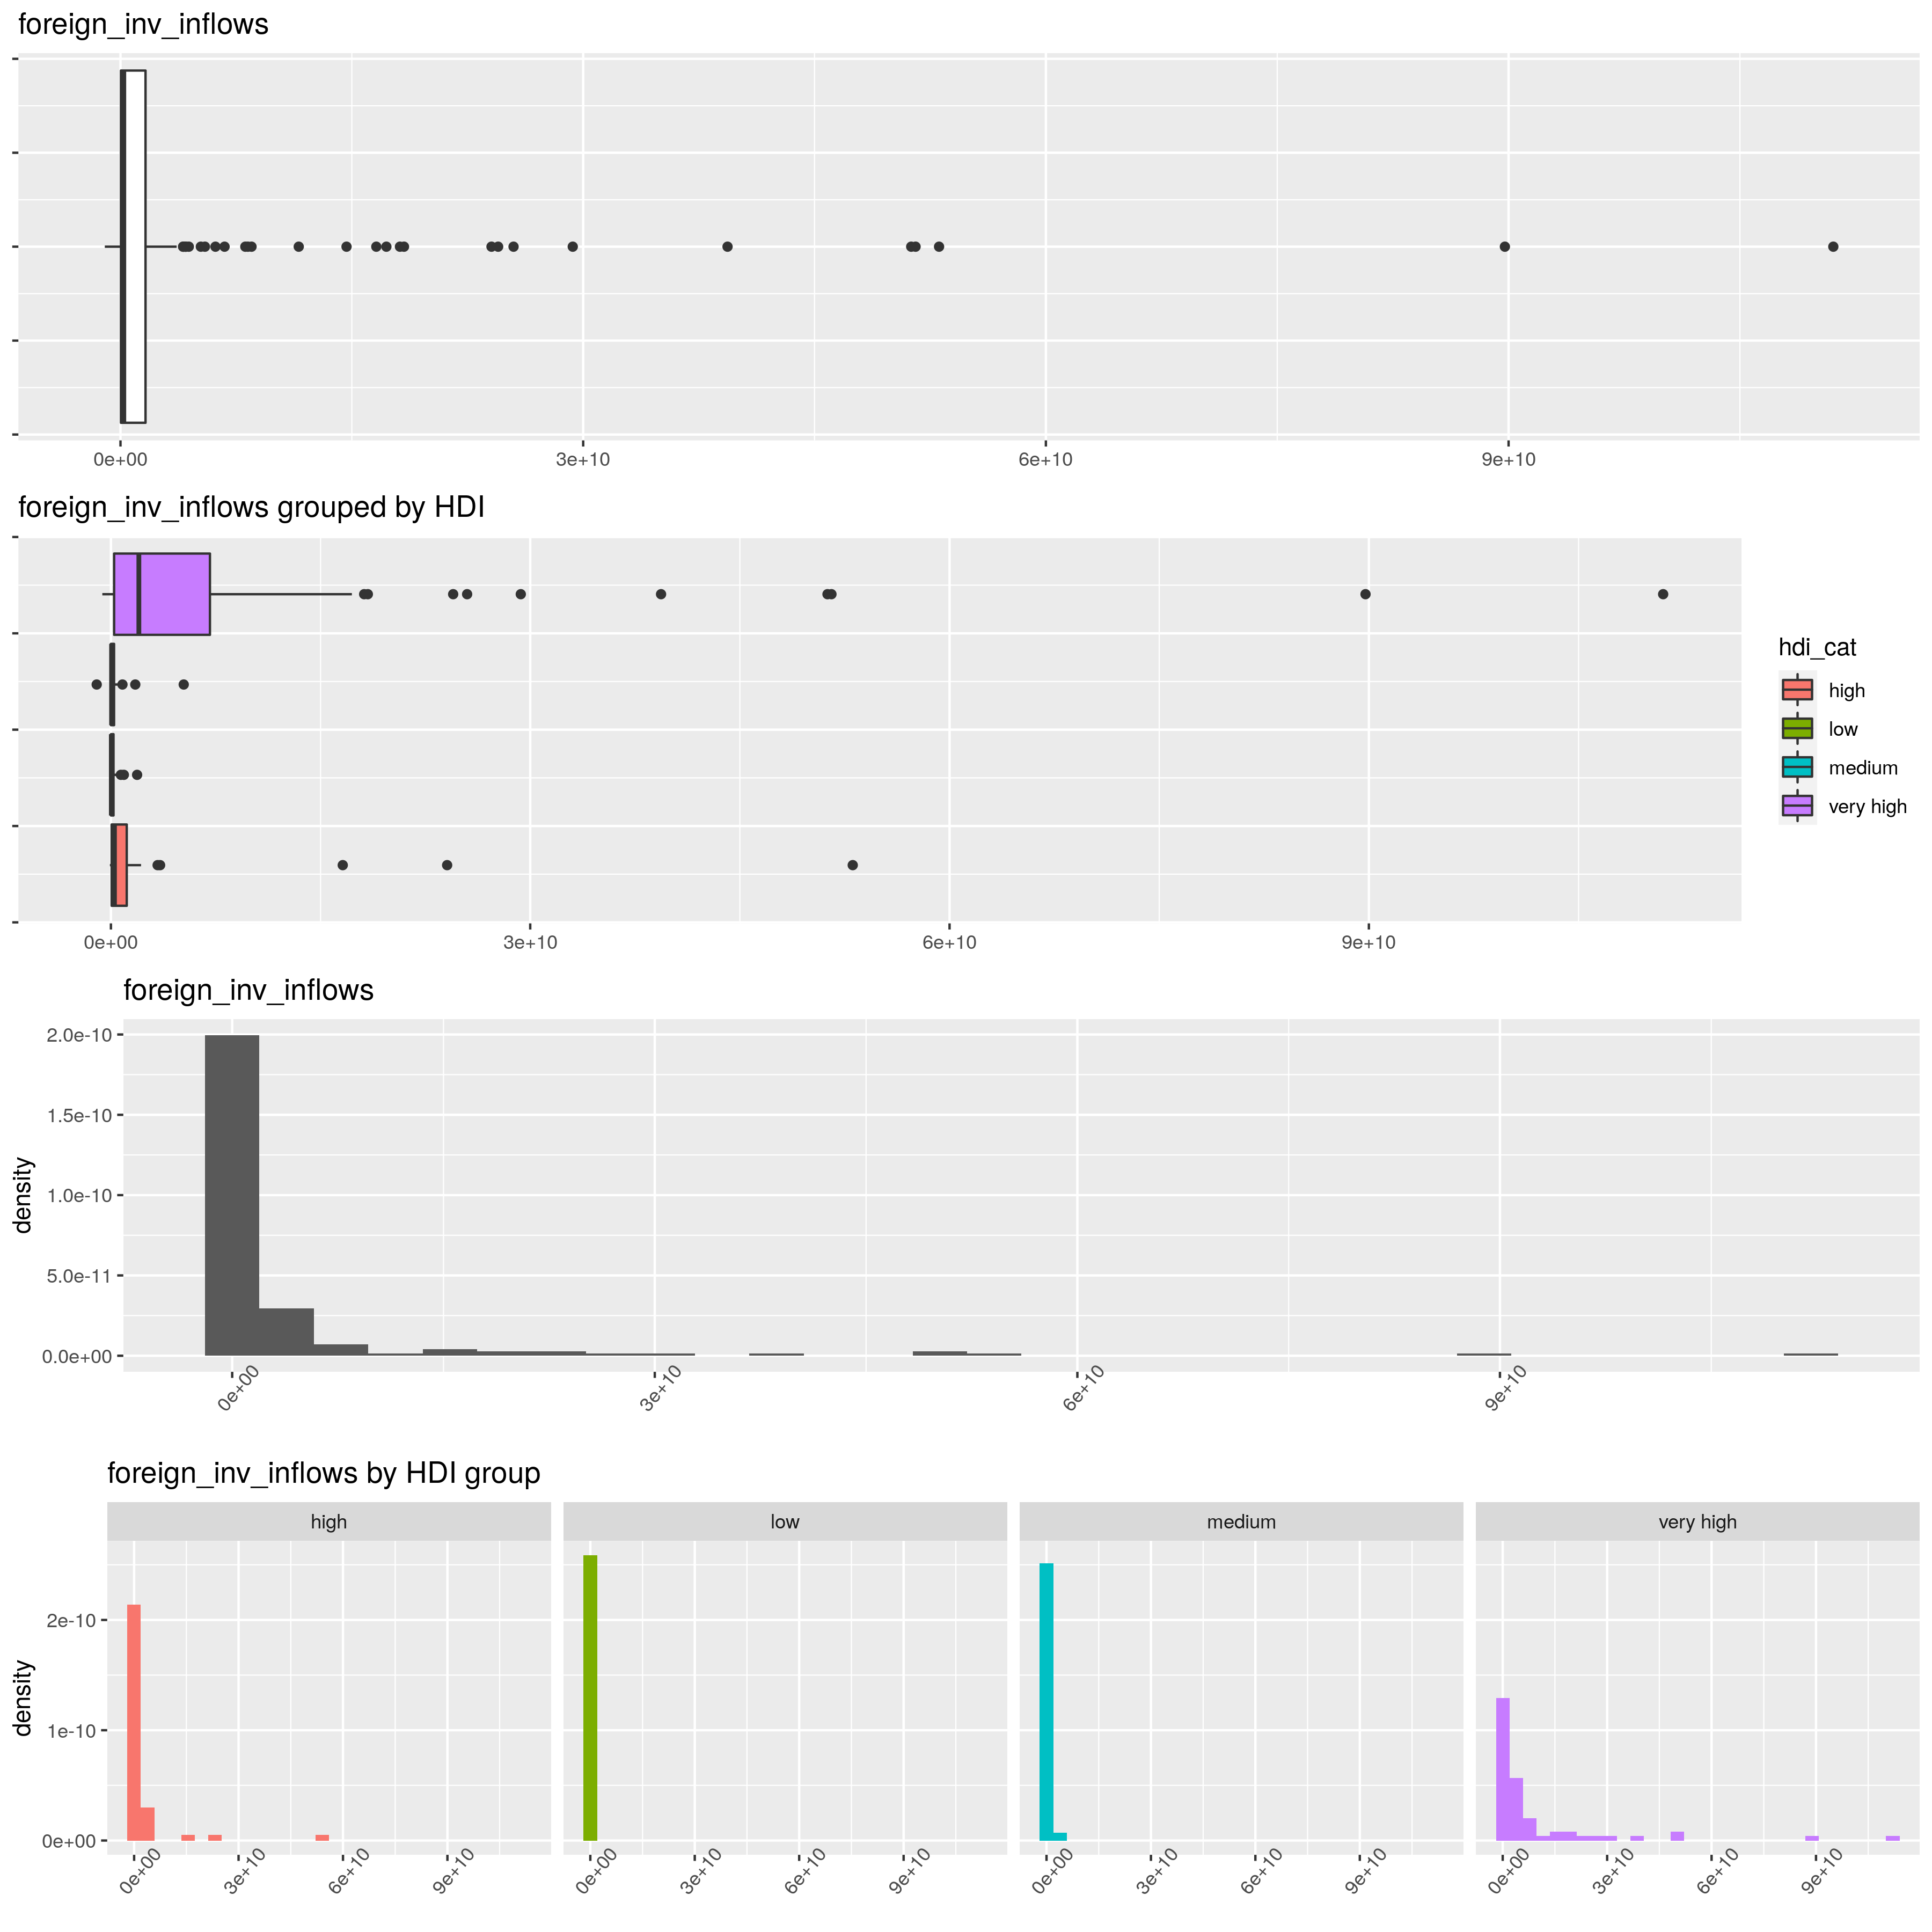
\includegraphics[width=0.6\textwidth,height=\textheight]{./img/foreign_inv_inflows.png}
\caption{Foreign Investment Inflows}
\end{figure}

The following variables showed a similarly right-skewed shape with
significant outliers:

\begin{itemize}
\tightlist
\item
  \textbf{foreign\_inv\_inflows}: Heavily right skewed, significant
  outliers (USA, UK, Germany, China\ldots{}) etc\ldots{} Given the
  histogram of \emph{foreign\_inv\_inflows} when grouped by very high
  HDI vs low HDI, it would seem like the more developed a country is,
  the more foreign investment it should have. The grouped boxplot also
  shows the same trend.
\item
  \textbf{int\_tourism\_receipts} and \textbf{int\_tourism\_arrivals}:
  Basically the same as with \emph{foreign\_inv\_inflows}, we see that
  there's a significant tendency for higher development nations to
  receive significantly more tourism receipts and arrivals.
\item
  \textbf{greenhouse\_gas\_em}: Just like with the previous two
  variables, fossil fuel use, meat production and economic activities
  like such produce huge amounts of greenhouse gases, and the more
  developed a country is, the more emissions it produces. However, this
  one is a bit less strongly inclined like the previous two. We can
  clearly see that there's many less developed countries with a high
  level of emissions. A notorious example of this is China, which is the
  2nd country with the most emissions and falls under the high category
  of HDI, by far exceeding the emission levels of most countries with
  very high HDI countries.
\end{itemize}

\hypertarget{education-variables}{%
\subsubsection{Education variables}\label{education-variables}}

\begin{figure}
\centering
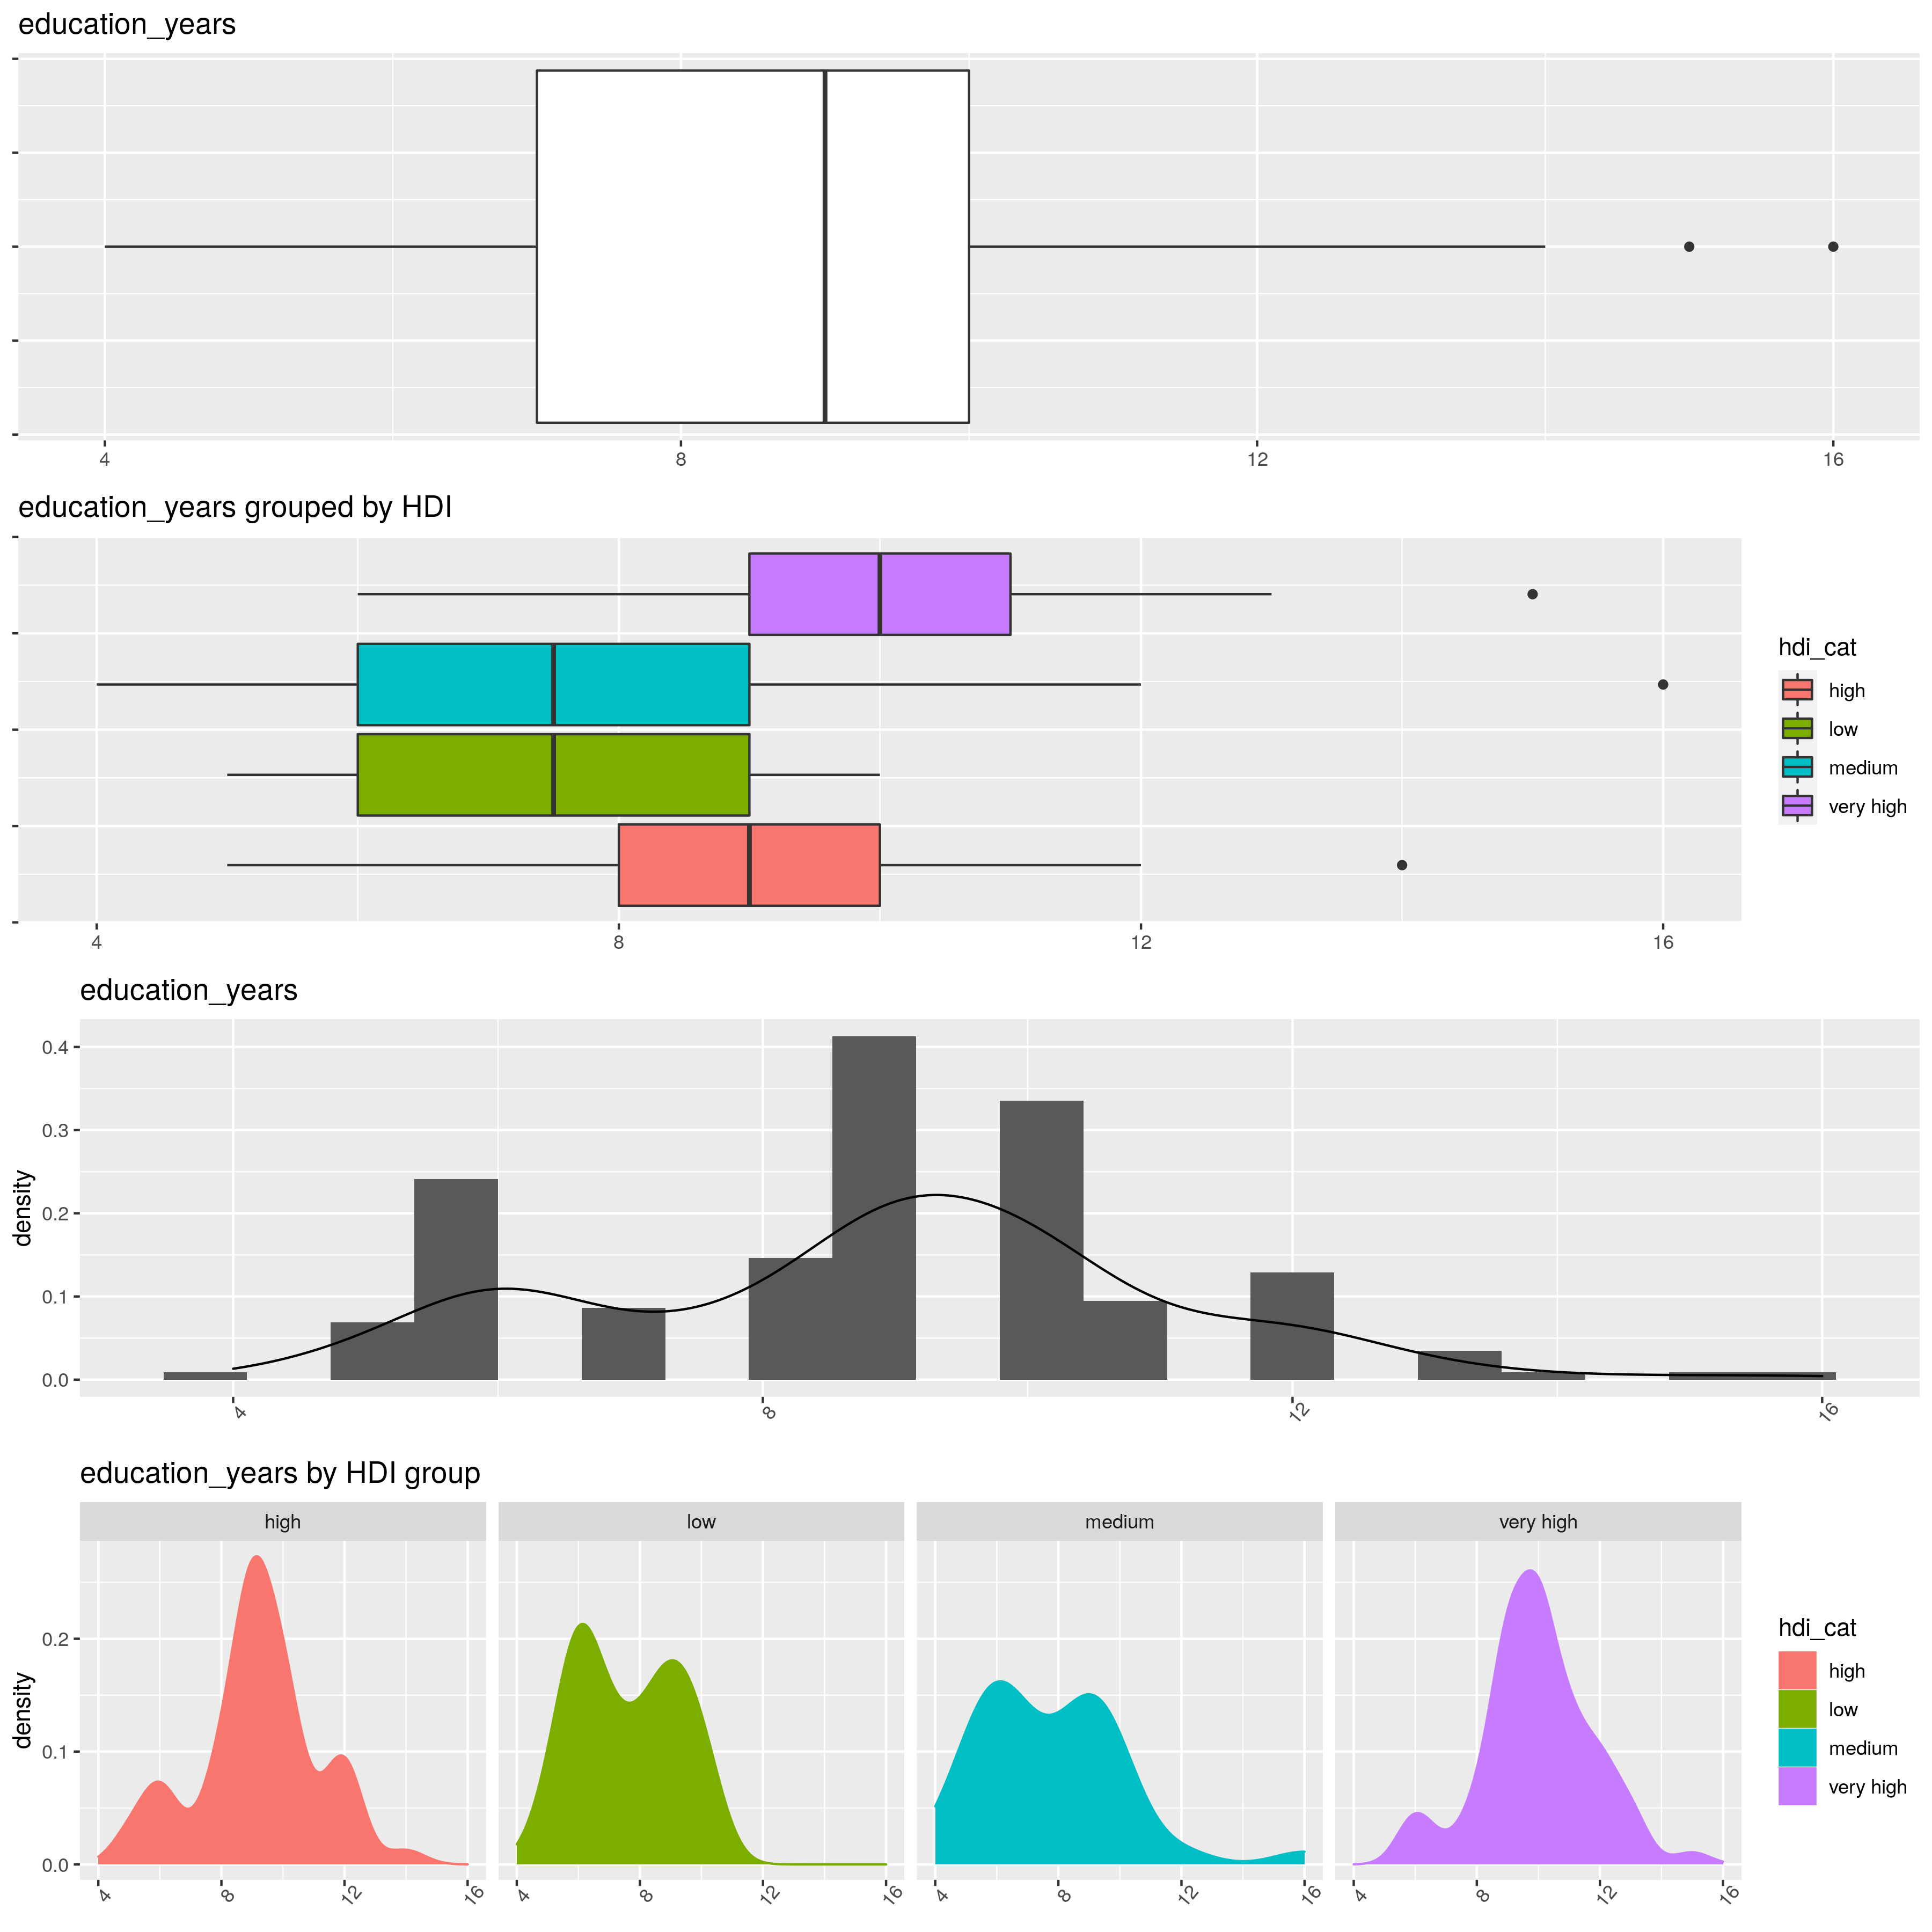
\includegraphics[width=0.6\textwidth,height=\textheight]{./img/education_years.png}
\caption{Years of compulsory education}
\end{figure}

\begin{itemize}
\tightlist
\item
  \textbf{education\_years}: There's a clear tendency, both shown by our
  grouped boxplots and grouped density plots, for very high HDI
  countries to have significantly longer periods compulsory education,
  with few exceptions in each group, however a clear tendency that peaks
  between 8 and 12 years of education for both high and very high HDI
  countries. Low and medium HDI countries could be clumped together with
  similar compulsory education times, but with more variability for
  medium HDI countries.
\item
  \textbf{education\_perc\_gdp}: How much are countries spending on
  education as a percentage of their GDP is a very interesting variable,
  as we can see that the consistency for higher and lower spendings
  respectively for low and very high HDI countries is quite solid, while
  medium HDI countries show an incredible variability versus other
  groups. High HDI countries show significant variability versus that of
  very high and low HDI countries, however, still aligning more iwth
  very high HDI countries than the rest.
\end{itemize}

\hypertarget{other-economic-variables}{%
\subsubsection{Other economic
variables}\label{other-economic-variables}}

These variables might have some skewness towards more tails or longer
tails than a normally distributed variable should have. Therefore
they're hard to classify as particularly right or left skewed.

\begin{itemize}
\tightlist
\item
  \textbf{exports\_perc\_gdp}: This variable has a long left tail and it
  is right-skewed. We can see the box for medium developed countries is
  larger than others while very high and high HDI countries tend to have
  higher export amounts as percentage of GDP. Low HDI countries lag
  behind, as expected. It is interesting to see how medium HDI countries
  completely bridge the gaps between high, very high and low HDI
  countries in terms of exports, in the sense that there's plenty of
  countries with medium HDI with exports just as high as others with
  significantly higher HDIs.
\item
  \textbf{inflation\_perc}: For inflation we can see that independently
  of the HDI of a country, inflation could, perhaps, be an inevitable
  event of economic/political management or mismanagement and
  uncertainty. Either way, we can clearly see that the higher the HDI,
  the less uncertain such inflation rate will be. The boxes for medium
  and low HDI countries are significantly larger than very high and high
  therefore telling us that there's less consistency and high inflation
  events, while universal, are unpredictable, but less unpredictable and
  probably less common the higher the HDI of a country is.
\item
  \textbf{gds\_perc\_gdp}: For gross domestic savings we can see that
  there's a clear difference between groups, with much more overlapping
  on the high end of HDI than the medium to low end of HDI. However,
  clearly, once again, the higher the HDI the higher the GDS. Much more
  variability again on those middle HDI groups (high and medium).
\item
  \textbf{gross\_savings\_perc\_gdp}: Gross savings as a percentage of
  GDP is an interesting variable, where the only defining feature of
  high and very high HDI countries being, again, relative consistency
  versus other groups, there might be seemingly no predictive capability
  in it due to the extremely lo variability of the values among groupsm
  however, it definitely differentiates very high and low HDI countries
  quite well.
\end{itemize}

\hypertarget{other-interesting-variables}{%
\subsubsection{Other interesting
variables}\label{other-interesting-variables}}

These variables seemed like quite appropriate to me for predicting HDI
or any other development measure, as they could potentially be huge
differentiators between the different HDI groups.

\begin{figure}
\centering
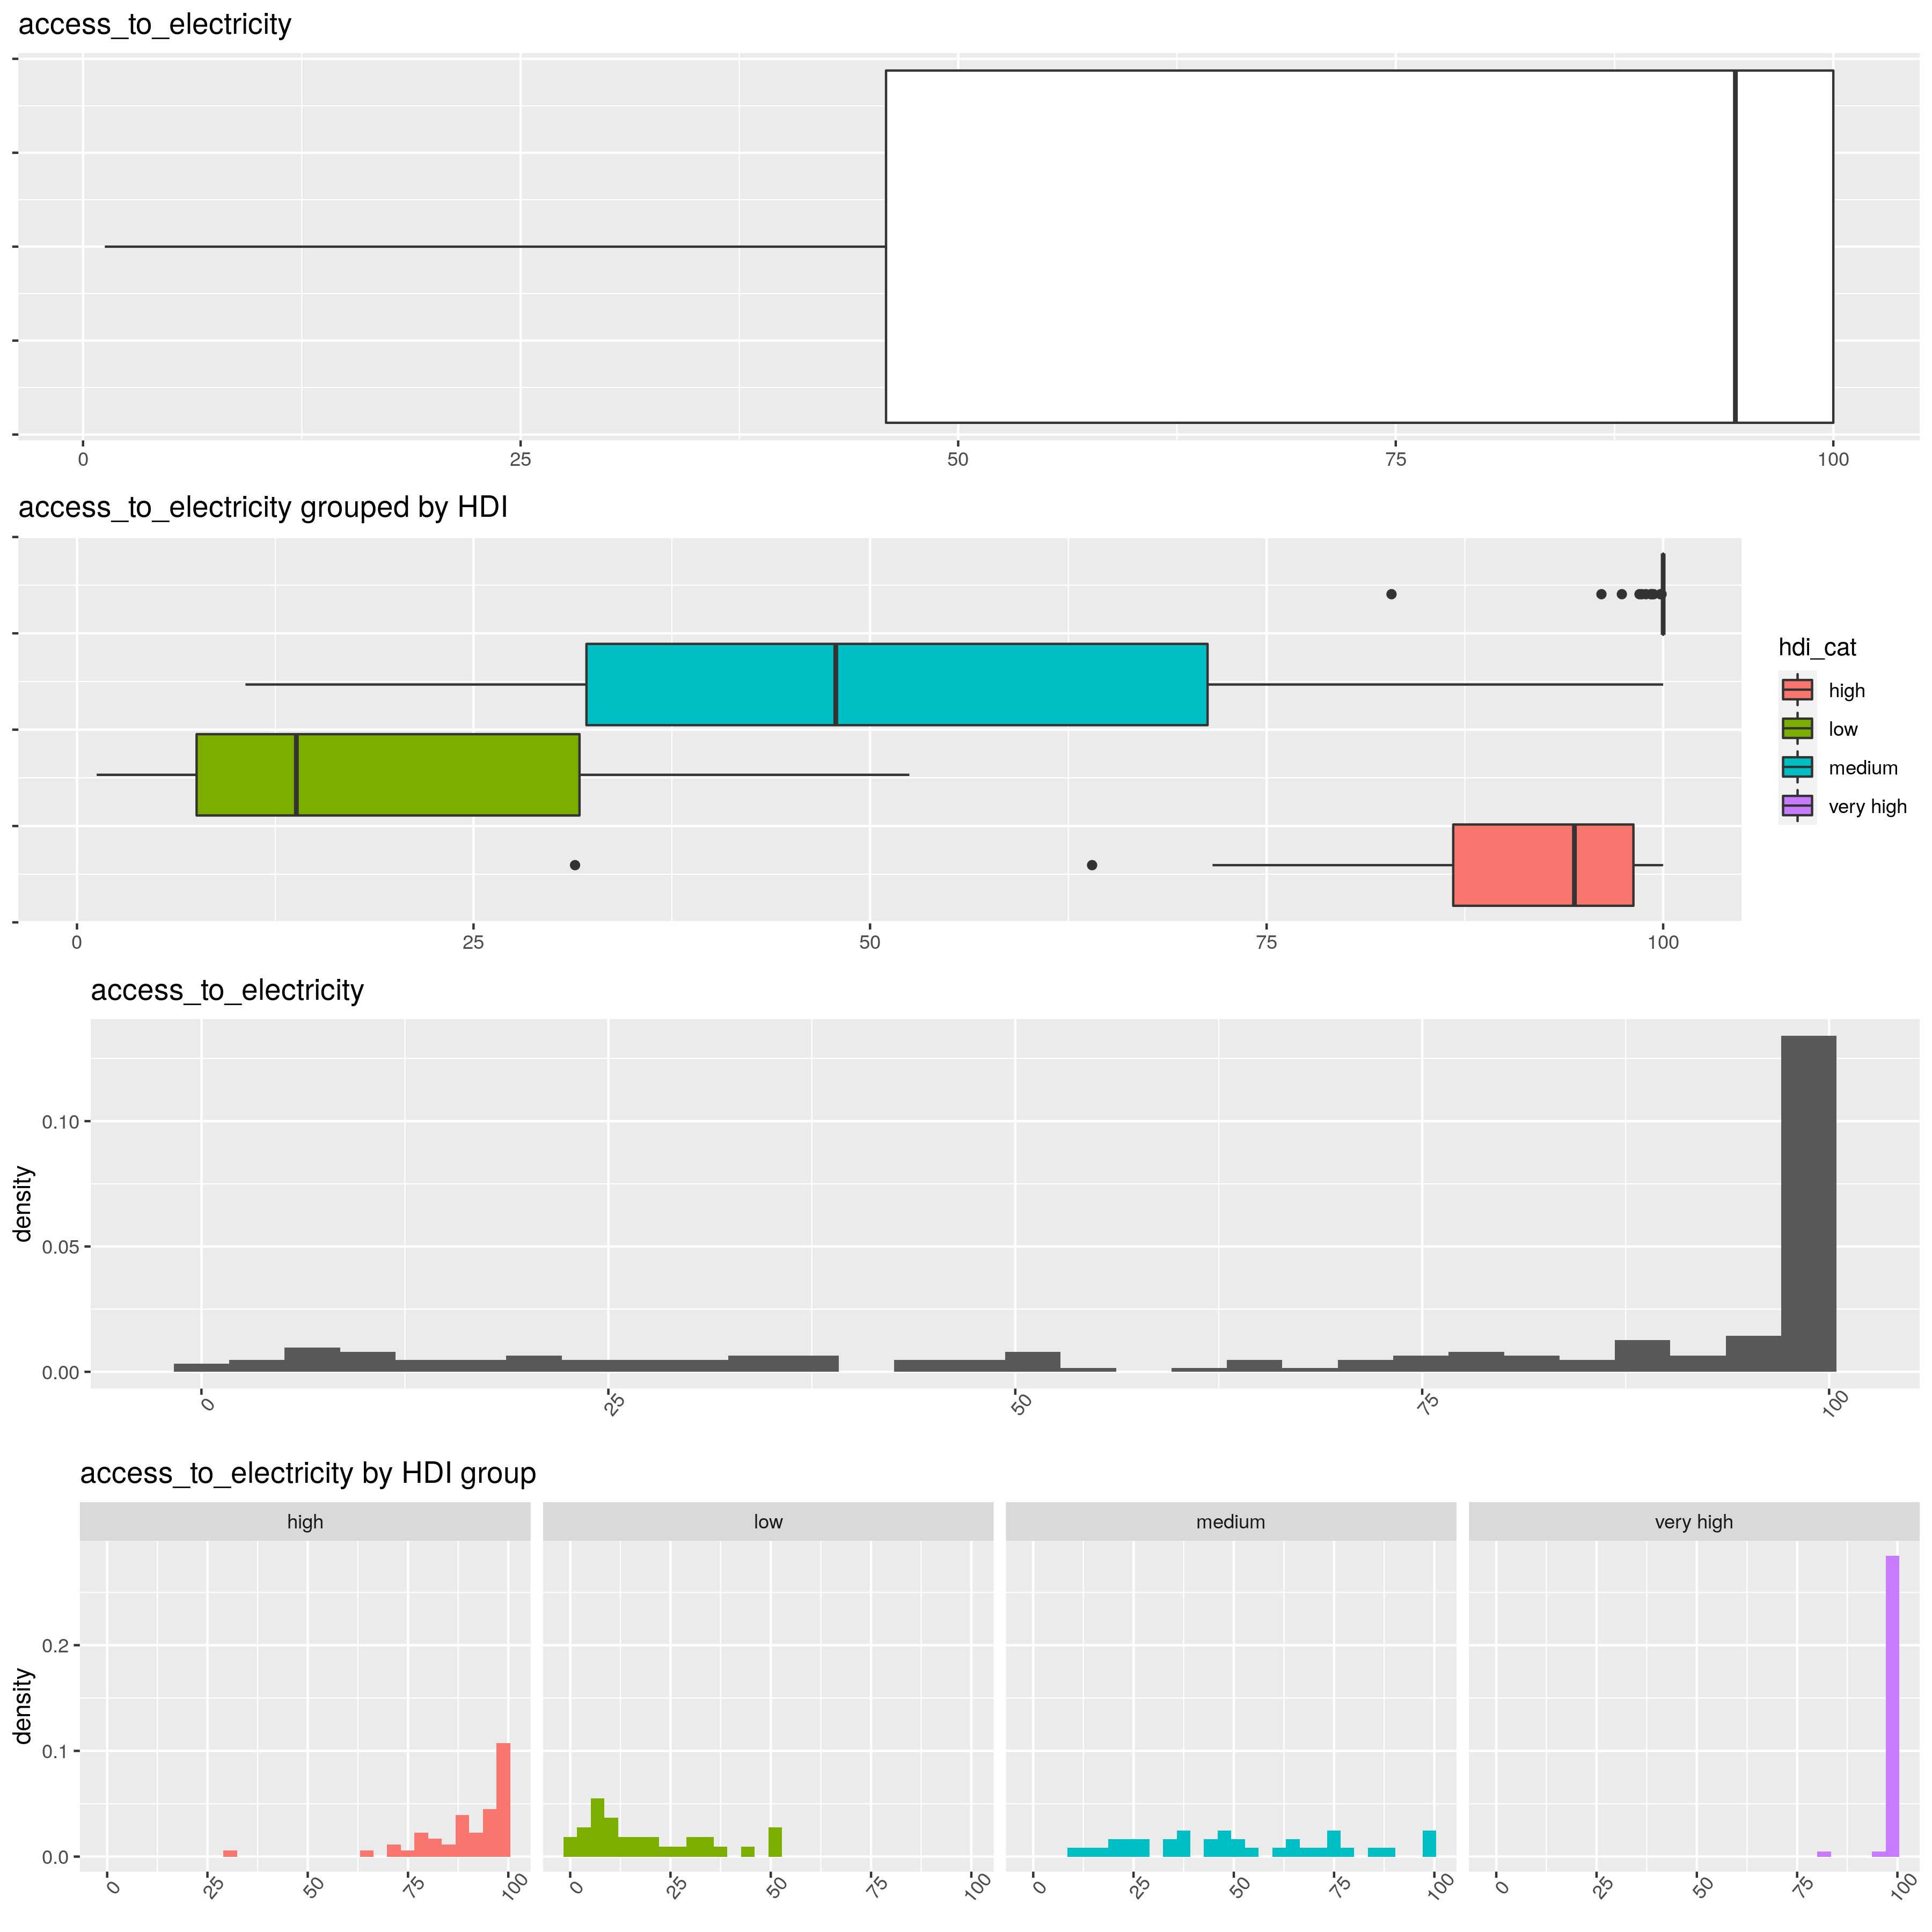
\includegraphics[width=0.6\textwidth,height=\textheight]{./img/access_to_electricity.png}
\caption{Percentage of population with access to electricity}
\end{figure}

\begin{itemize}
\tightlist
\item
  \textbf{perc\_internet\_users}: The percentage of internet users in
  each group is a surprisingly good differentiator as mentioned
  previously. We can see that, sure there's countries in each group with
  percentages that resemble other groups, but the difference in
  variability among groups is massive. Where the consistency of low HDI
  countries vs very high and high HDI countries is significantly
  different. We can see the standard deviations (and means) per group
  follow an interesting ladder: \(\sigma_{low} \approx 0.714\),
  \(\sigma_{medium} \approx 2.532\), \(\sigma_{high} \approx 4.908\),
  \(\sigma_{very\_high} \approx 20.382\).
\item
  \textbf{access\_to\_electricity}: another Hugely differentiating
  variable with similar properties to \emph{perc\_internet\_users}. We
  can see a clear division where if the country is in the very high HDI
  category, it will almost certainly have near full coverage in its
  electricity supply to its population. Countries in the high category
  are also clearly differentiated with the rest while also maintaining
  quite high rates. Medium HDI countries show a huge variability in
  their coverage, lower than high HDI countries but higher than low HDI
  countries. Low HDI countries show a significantly lower but clearly
  divided coverage with medium HDI countries.
\item
  \textbf{agricultural\_land}:
\end{itemize}

\end{document}
